
\documentclass[../projekt.tex]{subfiles}
\begin{document}


\section{Návrh serverovej časti}\label{navrhServer}
V~tejto kapitole sa zaoberám návrhom implementácie webového servera pre systém Fitcrack. Ako implementačné prostredie som zvolil Python3. Pri jeho výbere som bral v~úvahu už zaužívané technológie v~systéme Fitcrack, požadovanú funkčnosť systému a taktiež jeho prenositeľnosť.

\subsection{Rozdelenie systému na moduly}
Pre lepšiu organizáciu som celý systém rozdelil do niekoľko modulov (viď obr. \ref{fig:moduly}). Jednotlivé moduly sú detailnejšie rozobrané v~nasledujúcich podkapitolách. 

\begin{figure}[h]
    \label{fig:moduly}
    \centering
    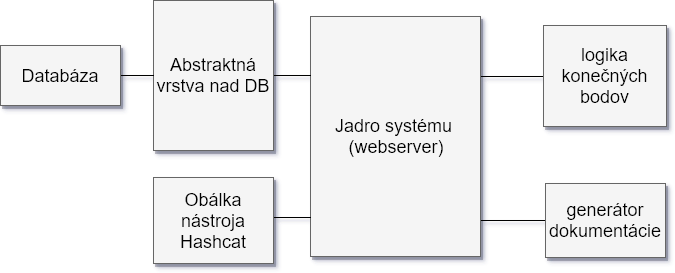
\includegraphics[scale=0.6]{obrazky/moduly.png}
    \caption{Rozdelenie systému do modulov}
\end{figure}

\subsubsection{Jadro systému}
Najhlavnejším modulom v~systéme je jeho jadro, ktoré spĺňa úlohu webového servera a sú v~ňom uložené nastavenia celého systému (prístupové údaje do databázy, zložka pre nahrávanie súborov, cesta k~nástroju Hashcat atď.). Pri zlyhaní jadra webový server odpovedá HTTP správy s~kódom začínajúcim číslom 5 (viď \ref{5XX}).


\subsubsection{Logika konečných bodov}
Jedná sa o~modul, v~ktorom sú obslúžené dotazy na konkrétne URI adresy. Zoznam dostupných URI je uvedený v~tabuľke \ref{zoznamURItable}. Pri chybe v~tomto module, webový server odpovedá HTTP správami, ktoré začínajú číslom 4 (viď \ref{4XX}). Ak užívateľ žiada o~neplatnú kombináciu URI adresy a HTTP metódy, je mu vrátená HTTP správa s~kódom 404. V~prípade že je užívateľ neprihlásený a žiada o~zdroj, ktorý vyžaduje autentifikáciu, v~odpovedi dostane HTTP správu s~kódom 401. Pokiaľ je užívateľ prihlásený, ale na zdroj o~ktorý žiada nemá dostačujúce oprávnenia, tento modul vracia HTTP správu s~kódom 403. V~inakšom prípade je dotaz týmto modulom spracovaný. Ak nedôjde k~chybe počas spracovávania dotazu, modul vygeneruje odpoveď vo formáte JSON, ktorú pridá do tela HTTP odpovede s~kódom 200 (viď \ref{2XX}).


\begin{table}[h]
	\begin{center}
        \begin{tabular}{ |p{7.7cm}|p{4.9cm}|p{1.5cm}|  }
         \hline
         \multicolumn{3}{|c|}{Jednotlivé URI adresy} \\
         \hline
         Názov služby& URI& Metóda\\
         \hline
         Prihlásenie užívateľa& /user/login & POST\\
         Registrácia užívateľa& /user/register& POST\\
         Odhlásenie užívateľa& /user/logout& GET\\
         Zoznam podporovaných hešov & /hashTypes & GET\\
         Zoznam podporovaných typov útokov & /attackModes & GET\\
         Zobrazenie kolekcie balíkov & /package & GET\\
         Pridať balík & /package & POST\\
         Zmazať balík & /package/\{packageID\} & DELETE\\
         Upraviť balík & /package\{packageID\} & UPDATE\\
         Zobrazí podrobné informácie o~balíku& /package/\{packageID\} & GET\\
         Operácia nad balíkom (reštart, štart, stop) & /package/\{packageID\}/action & POST\\
         Vráti kolekciu úloh, na ktoré je balík rozdelený& /package/\{packageID\}/job & GET\\
         Zobrazí hosťov, ktorí sú pridelení k~balíku & /package/\{packageID\}/host & GET\\
         Pridá hostí k~balíku & /package/\{packageID\}/host & POST\\
         Odoberie hostí z~práce na balíku & /package/\{packageID\}/host & DELETE\\
         Zobrazí kolekciu hostí& /host & GET\\
         Deaktivuje konkrétneho hosťa& /host/\{hostID\} & DELETE\\
         Vráti kolekciu slovníkov& /dictionary & GET\\
         Vráti obsah konkrétneho slovníka& /dictionary/\{dictionaryID\} & GET\\
         Vymaže slovník zo systému& /dictionary/\{dictionaryID\} & DELETE\\
         Informácie o~serveri& /server/info& GET\\
         Operácia so serverom (reštart, štart, stop) & /server/action & POST\\
         \hline
        \end{tabular}
  		\caption{Zoznam dostupných URI.}
  		\label{zoznamURItable}
	\end{center}
\end{table}

\subsubsection{Obálka nástroja Hashcat}
Aj keď serverová časť systému Fitcrack nepoužíva priamo nástroj Hashcat na generovanie hešov kryptografických funkcií, používa ho na rôzne vedľajšie účely, ako napríklad získavanie podporovaných typov útokov a kryptografických hešov. Z~tohto dôvodu je potrebné implementovať obálku na tento nástroj vo forme objektu (triedy) s~požadovanými funkciami. To nám uľahčí prístup k~nástroju Hashcat a taktiež bezpečnejšie narábanie s~ním.

\subsubsection{Abstraktná vrstva nad databázou}
Jedná sa o~modul, ktorý výrazne uľahčuje prístup k~databáze. Zároveň výrazne neovplyvňuje výkon a flexibilitu systému. Vďaka tomu, že systém s~databázou nekomunikuje priamo, ale využíva abstraktnú vrstvu, je databáza lepšie chránená (ochrana pred útokmi typu SQL injection).


\subsubsection{Databáza}
Vzhľadom nato, že systém Fitcrack využíva databázový server MySQL, rozhodol som sa napojiť na túto databázu. Aby bolo možné implementovať všetky rozšírenia systému, bude potrebné modifikovať štruktúru databázy.


\subsubsection{Generátor dokumentácie}
Generátor dokumentácie po spustení webového servera spracuje zdrojové kódy aj s~komentárami a vytvorí pomocou nich interaktívnu dokumentáciu (viď obr. \ref{fig:doc}). Z~nej je potom možné zistiť všetky dostupné koncové body spolu s~príkladmi odpovede. Generovanie dokumentácie automaticky nastáva aj pri zmene zdrojových súborov.

\begin{figure}[H]
    \centering
    \label{fig:doc}
    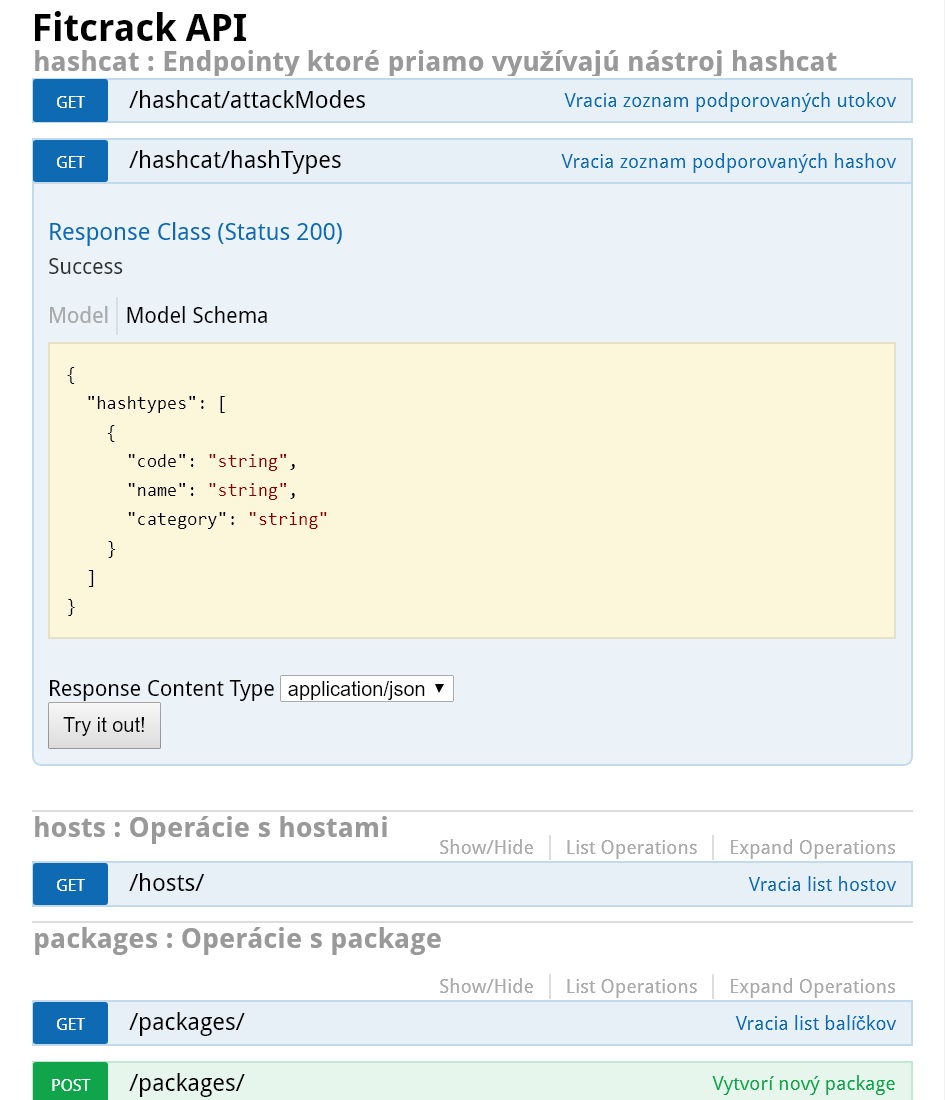
\includegraphics[scale=0.45]{obrazky/doc.PNG}
    \caption{Ukážka vygenerovanej dokumentácie}
\end{figure}

\subsection{Autentifikácia a oprávnenia užívateľov}
Súčasný systém Fitcrack nepodporuje viacerých užívateľov. Aby bolo možné toto vylepšenie implementovať, je potrebné do databázy pridať tabuľku \texttt{fc\_users}. Okrem mena užívateľa a zahešovaného hesla táto tabuľka obsahuje užívateľský email a všeobecné právomoci užívateľa na serveri. Jedná sa o~číslo, ktoré čím je väčšie, tým väčšie má právomoci užívateľ. Napríklad ak má užívateľ v~stĺpci \texttt{competence\_level} číslo 9, môže pridávať do systému nové užívateľské účty, robiť operácie so serverom (napríklad reštart), a vidieť všetky balíčky ktoré sa v~systéme nachádzajú. Oproti nemu, užívateľ so všeobecnými oprávneniami nastavenými na 1, nemôže pridávať nových užívateľov, ani vykonávať operácie so serverom a má prístup len k~balíčkom, ktoré sú mu pridelené.

Pre jednoduchšiu implementáciu oprávnení užívateľov k~balíkom som pridal ďalšiu tabuľku \texttt{fc\_permissions} ( upravená štruktúra databázy je zobrazená na obrázku \ref{fig:db}). Základné oprávnenia užívateľa k~balíku sú tri. Najzákladnejšie oprávnenie dovoľuje užívateľovi vidieť balík medzi kolekciou balíkov, a zároveň zobraziť detailné informácie o~balíku. Ďalšie oprávnenie dovoľuje užívateľovi vykonávať operácie s~balíkom (štart, stop, reštart a úprava hosťov, ktorí sa podieľajú na balíku). Posledné oprávnenie dovoľuje užívateľovi vymazať balík z~databázy.

\begin{figure}[h]
    \centering
    \label{fig:db}
    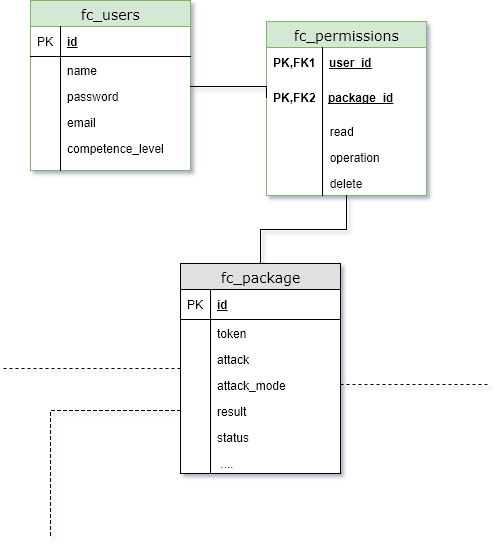
\includegraphics[scale=0.6]{obrazky/users.png}
    \caption{Časť entitno - relačného diagramu databázy systému Fitcrack. Tabuľky označené zelenou farbou sú nové.}
\end{figure}


\end{document}

